%!TEX TS-program = xelatex
%!TEX encoding = UTF-8 Unicode

%%%%%%%%%%%%%%%%%%%%%%%%%%%%%%%%%%%%%%%%%
% Journal Article
% LaTeX Template
% Version 1.4 (15/5/16)
%
% This template has been downloaded from:
% http://www.LaTeXTemplates.com
%
% Original author:
% Frits Wenneker (http://www.howtotex.com) with extensive modifications by
% Vel (vel@LaTeXTemplates.com)
%
% License:
% CC BY-NC-SA 3.0 (http://creativecommons.org/licenses/by-nc-sa/3.0/)
%
%%%%%%%%%%%%%%%%%%%%%%%%%%%%%%%%%%%%%%%%%

%----------------------------------------------------------------------------------------
%	PACKAGES AND OTHER DOCUMENT CONFIGURATIONS
%----------------------------------------------------------------------------------------

\documentclass[
	12pt,
	a4paper,
	%twoside,
	twocolumn
	]{article}

\usepackage{blindtext} % Package to generate dummy text throughout this template

%\usepackage[sc]{mathpazo} % Use the Palatino font
\usepackage[T1]{fontenc} % Use 8-bit encoding that has 256 glyphs
\usepackage[utf8]{inputenc}

\linespread{1.05} % Line spacing - Palatino needs more space between lines
\usepackage{microtype} % Slightly tweak font spacing for aesthetics

\usepackage[english]{babel}

\usepackage[
	%hmarginratio=1:1,
	top=20mm,
	bottom=20mm,
	textwidth=17.2cm,
	columnsep=0.8cm%19pt
	]{geometry} % Document margins

%-------------------------------------------------------------
%----------------------------------------------------- FONTS -
%-------------------------------------------------------------

\linespread{1.04}

\usepackage{paralist}

\usepackage{etoolbox}

\usepackage{fontspec,
			xltxtra,
			xunicode
			}

\defaultfontfeatures{Mapping=tex-text}

\setromanfont[
	Mapping=tex-text
	]{Alegreya}

\setsansfont[
	Scale=MatchLowercase,
	Mapping=tex-text,
	% LetterSpace=3.0,
	% Scale=0.707,
	]{Fira Sans}

\setmonofont[]{Fira Mono}

\newfontfamily{\scaps}{Alegreya SC}

\newfontfamily\quotefont[
	Scale=MatchLowercase,
	Mapping=tex-text,
	LetterSpace=3.0,
	%Scale=1.123,
	]{Fira Sans}
\AtBeginEnvironment{quote}{\quotefont\small}

\usepackage{lilyglyphs}
\usepackage{graphicx,dblfloatfix}

\usepackage[
	hang,
	small,
	labelfont=bf,
	up,
	textfont=it,
	up
	]{caption}

\usepackage{booktabs} % Horizontal rules in tables

\usepackage{lettrine} % The lettrine is the first enlarged letter at the beginning of the text

\usepackage{enumitem} % Customized lists
\setlist[itemize]{noitemsep} % Make itemize lists more compact

\usepackage{abstract} % Allows abstract customization
\renewcommand{\abstractnamefont}{\normalfont\bfseries} % Set the "Abstract" text to bold
\renewcommand{\abstracttextfont}{\normalfont\small\itshape} % Set the abstract itself to small italic text

\usepackage{titlesec} % Allows customization of titles
\renewcommand\thesection{\Roman{section}} % Roman numerals for the sections
\renewcommand\thesubsection{\roman{subsection}} % roman numerals for subsections
\titleformat{\section}[block]{\large\scshape\centering}{\thesection.}{1em}{} % Change the look of the section titles
\titleformat{\subsection}[block]{\large}{\thesubsection.}{1em}{} % Change the look of the section titles

\usepackage{fancyhdr} % Headers and footers
\pagestyle{fancy} % All pages have headers and footers
\fancyhead{} % Blank out the default header
\fancyfoot{} % Blank out the default footer
\fancyhead[C]{\small Giuseppe Silvi • Thinking Tetrahedral Today} % Custom header text
\fancyfoot[RO,LE]{\thepage} % Custom footer text

\usepackage{titling} % Customizing the title section

\usepackage{hyperref} % For hyperlinks in the PDF

%----------------------------------------------------------------------------------------
%	TITLE SECTION
%----------------------------------------------------------------------------------------

\setlength{\droptitle}{-4\baselineskip} % Move the title up

\pretitle{\begin{center}\huge\bfseries} % Article title formatting
\posttitle{\end{center}} % Article title closing formatting
\title{Thinking Tetrahedral Today \\ \large{\emph{the rhythm perception of sound-shape in a four-dimensional space}}} % Article title
\author{%
\textsc{Giuseppe Silvi}\\[1ex]% \thanks{A thank you or further information} \\[1ex] % Your name
%\normalsize Conservatorio S. Cecilia di Roma \\ % Your institution
\normalsize \href{mailto:me@giuseppesilvi.com}{grammaton@me.com} % Your email address
%\and % Uncomment if 2 authors are required, duplicate these 4 lines if more
%\textsc{Jane Smith}\thanks{Corresponding author} \\[1ex] % Second author's name
%\normalsize University of Utah \\ % Second author's institution
%\normalsize \href{mailto:jane@smith.com}{jane@smith.com} % Second author's email address
}
\date{\today} % Leave empty to omit a date

\renewcommand{\maketitlehookd}{%
\begin{abstract}

%\noindent Short summary of the proposed project (max.100 words) including main objective, research questions, methods, and relevance to the research at RITMO.
\noindent\input{abstract.txt}

\end{abstract}
}

%----------------------------------------------------------------------------------------
%	DOCUMENT
%----------------------------------------------------------------------------------------

\begin{document}

\maketitle
%\raggedright
%----------------------------------------------------------------------------------------
\section*{RESEARCH OUTLINE}
%Background and theoretical framework 
%(Outline the theoretical foundation of your proposed research and why you have chosen this particular foundation.)
The \emph{spectromorphology} of sounds has deep roots in the sound analysis. \cite{smalley_1997} The research seam to the possibility of integrations of this knowledge with multi-dimensional sound reproduction technologies. \cite{fellgett_75, gerzon_70a, gerzon_70b} 

Each acoustical object has a complex propagation through space. This complexity combines multiple elements in a topological shape-space relationship, like pitch (or range of pitches), intensity, duration, directivity and, most of all, the perspective point of listening. 

These fundamentals concepts are the most vulnerable aspects of sound in mixed music live concert. At the same time, they are the key parameters of pure magic. When the time-space relationship between sources are balanced, the listener is projected elsewhere, and we are magicians.


\begin{figure}[htbp]
\centering
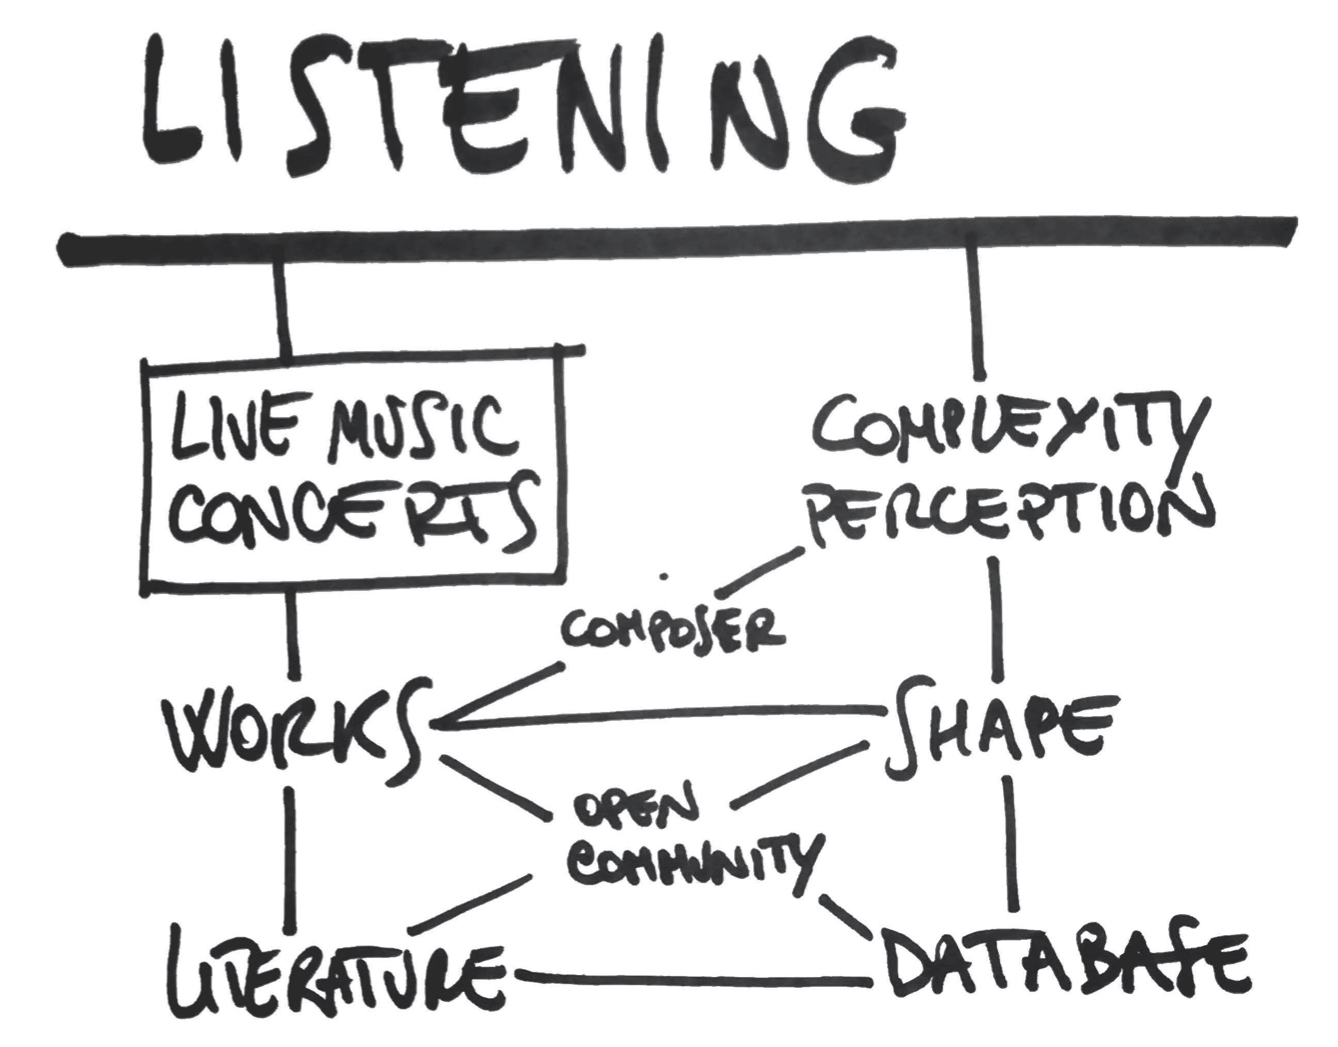
\includegraphics[width=.47\textwidth]{img/2020-01-20-14-20.jpg}
\caption{Research outline}
\label{outline}
\end{figure}

%----------------------------------------------------------------------------------------
\section*{MAIN OBJECTIVE, RESEARCH \\ QUESTIONS AND HYPOTESIS}
%(Present the objectives, questions and expected findings of the proposed project. Explain how your research will be relevant for RITMO.)
%
%It is expected that all members of the centre contribute to the general activities and collaborations within RITMO. The researchers have access to state-of-the-art facilities in sound/video recording, motion capture, eye tracking, physiological measurements, various types of brain imaging (EEG, fMRI), and rapid prototyping and robotics laboratories.
\emph{At the depth of every literature, the time.}

I consider the listener as time observer, I think about music as a memory game, as the composer speculation on time-relationship through the unknown listener mind. By this way, what happens in space, from the performance gesture to the activity of an observer, are precious time relationships to be discovered and explained.

The electroacoustic literature explains what the sound-shape is, mostly trough abstract conceptualizations. But it is truly observable even in the acoustic realm. It is the way we can figure the \emph{horn} sound and its differences to a \emph{bassoon} or different reverberated space around them. It is the plastic memory of the rhythm relationship.

To fully investigate it, a representation of the sound-shape is required. What approach to the sound-shape analysis of an acoustical object is more efficient? The efficiency of representation is necessary to focus on the relationship between these core fundamentals and the people's way of listening. It needs to be related to the real possibility of staging and it must produce a tangible solution for live music. 

Is it possible to reproduce a sound-shape and compare its electroacoustic reproduction with the acoustical one? Yes, it is possible. The simplest three dimensional solid is the tetrahedron. Through the diffusion of sound by its four faces, it is possible to obtain the simplest and more efficient sound-shape reproduction. 

What is the emotional impact of the micro-rhythm relationship amongst mixed sound-shapes during a live concert? This is the very unsolved question of my ten years personal research path. This is what I think attractive to RITMO necessity to my research and my contribution perspective. The net of facilities and sensibilities at RITMO could afford to stage of compositions thought fundamentals of this research, with precise strategies to map, to track, to analyze music written on the same core of data to be observed. The stage as half of the listening attitude. The research to seam both.

%----------------------------------------------------------------------------------------

\section*{METHOD}

\begin{quote}
Music is not only about composing. It’s not artisanship, neither only a craft. Music is the thought.\footnote{Originally in Italian, present author traduction.}\cite{nono85}.
\end{quote}

Those Luigi Nono's words explain the attitude of doing music with the inexorability of perception, which involves listening and thinking, and writing and speaking and changing idea. These activities are the rhythm of composing, the topologies of a musical idea. 

I wish to contribute, with my research and music, to establish a community thinking around relevant facts emerging by deep working on time fundamentals of perception. I wish my research to be open, not only in terms of the source accessibility but also as open experience accessible with listening. I wish people can sit to listen to music and I can discuss with them, stimulate their perspective to listen better.

My personal knowledge is strongly focused on sound analysis. I truly understand and wish the necessity to integrate other forms of analysis I supposed to learn, counting on RITMO facilities my technique could be expanded with motion-capture and multiple videos tracking, to seam gesture and shape in a multi-dimensional view. 

The technology to be adopted will focus on open-source media, like textual code for real-time DSP and web community accessible data.

%\vfill

\begin{figure}[htbp]
\begin{center}
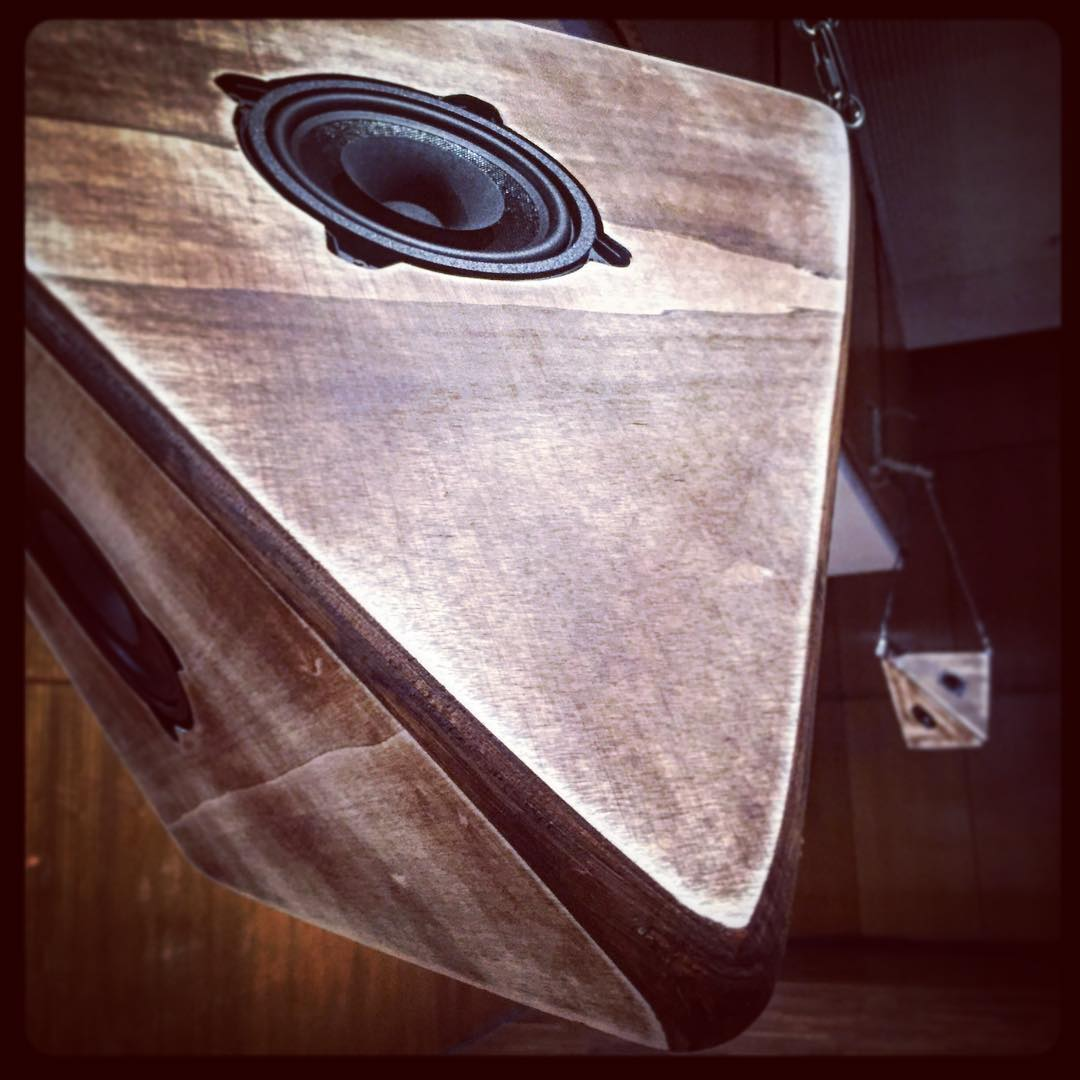
\includegraphics[width=.47\textwidth]{img/13556748_1807931906092757_1243460980_n.jpg}
\caption{S.T.ONE (Spherical Tetrahedral ONE) is the result of personal research aimed at balanced music staging between acoustical objects and electro-acoustics. The project permits to exploit the sound space created by the electronic medium with perceptive characteristics similar to traditional instruments. The directions and diffusions of sound are open-software controlled. The STONE project was never presented to the community.}
\label{stone2}
\end{center}
\end{figure}

%----------------------------------------------------------------------------------------
\section*{PROGRESS PLAN}

The presented research will be sliced into four stages. The first three phases will produce fundamentals basis of research. The last-one phase is the evidence of entire research in the form of the musical matter. It will produce final research documentation and music compositions to explore-expose the research through listening.

\begin{table}[htp]
\begin{center}
\begin{tabular}{ll}
\textbf{Phases} & \textbf{Dur.} \\
\hline
\textbf{Omnidirectional Expositions} & 6 mo. \\
Sound-shape analysis & \\
Sound-shape visualizations & \\
Sound-shape reproduction & \\
\hline
\textbf{Micro-Rhythm of sound-shape} & 6 mo. \\
Solo repertoire analysis & \\
Sound-shape explosion in practising & \\
From literature to shapes open-data & \\
\hline
\textbf{Rhythm of sound-shape interactions} & 12 mo. \\
Multiple sources multiple shapes & \\
Relationship and complexity perception & \\
\hline
\textbf{Musical compositions} & 12 mo. \\
UNISOLO: 4 ensembles and electronics & \\
Sound-shape in music composition & \\
MusicLab: unleashed opportunities & \\
Final documentation
\end{tabular}
\label{timesheet}
\caption{Thinking Tetrahedral Today phases}
\end{center}
\end{table}%

The first stage will produce the fundamentals of tetrahedral shape conceptualization to achieve the following objectives:

\begin{compactitem}
\item Capture the \textbf{sound-shape} of acoustical instruments
\item Preserve the \textbf{body shadow} on sound propagation
\item Preserve the \textbf{movements} performed by the musician
%\item Collect data of different acoustic instruments
%\item Collect data of different performers
\item Analyse data to prototype a \textbf{graphic visualisation}
\item Capture sounds for \textbf{point of view} listening (POL)
\item Collect music for virtual-reality environment
\end{compactitem}

%\vfill

\begin{figure}[htbp]
\begin{center}
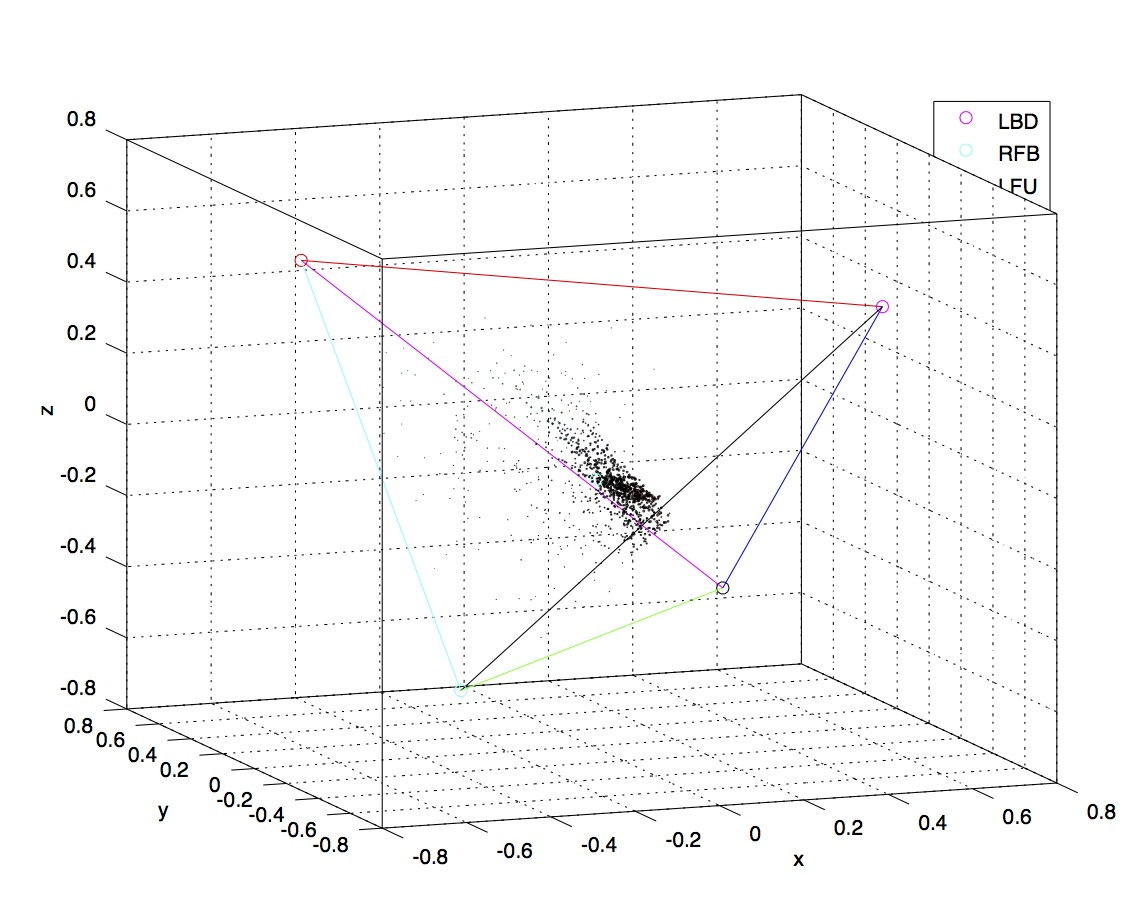
\includegraphics[width=.47\textwidth]{img/13230_1024_2.jpg}
\caption{A flute sound-shape visualization in four-dimensional space}
\label{shape}
\end{center}
\end{figure}

%\clearpage

%I wish to approach to motion and video capture of the performance to build a monolithic, multi-dimensional thought of shape.

The second stage will develop fundamentals through the analysis of acoustical behaviour of the musical instruments by timbral exploration, with the evidence of the micro-formal, time-related, explosion of shape through instrumental investigation.

The third stage is about complexity perception. The sound-shape stands out in the surrounding space and expands and moves within this space, modelled by it as a soft mass inside a container. Here the phenomena of reflection occur and the shape crystallizes assuming characteristics in the function of space and, therefore, of time. The listener who takes part in this event sees a solid instrument sounds in space. S/He feels the solid shape coming from the instrumental body and from the room in terms of reflections. A ritual, the one of listening, which can not do without any of these details. This stage has a lot of unanswered questions and, I wish, even a lot of not even issued too. 

\begin{figure}[htbp]
\begin{center}
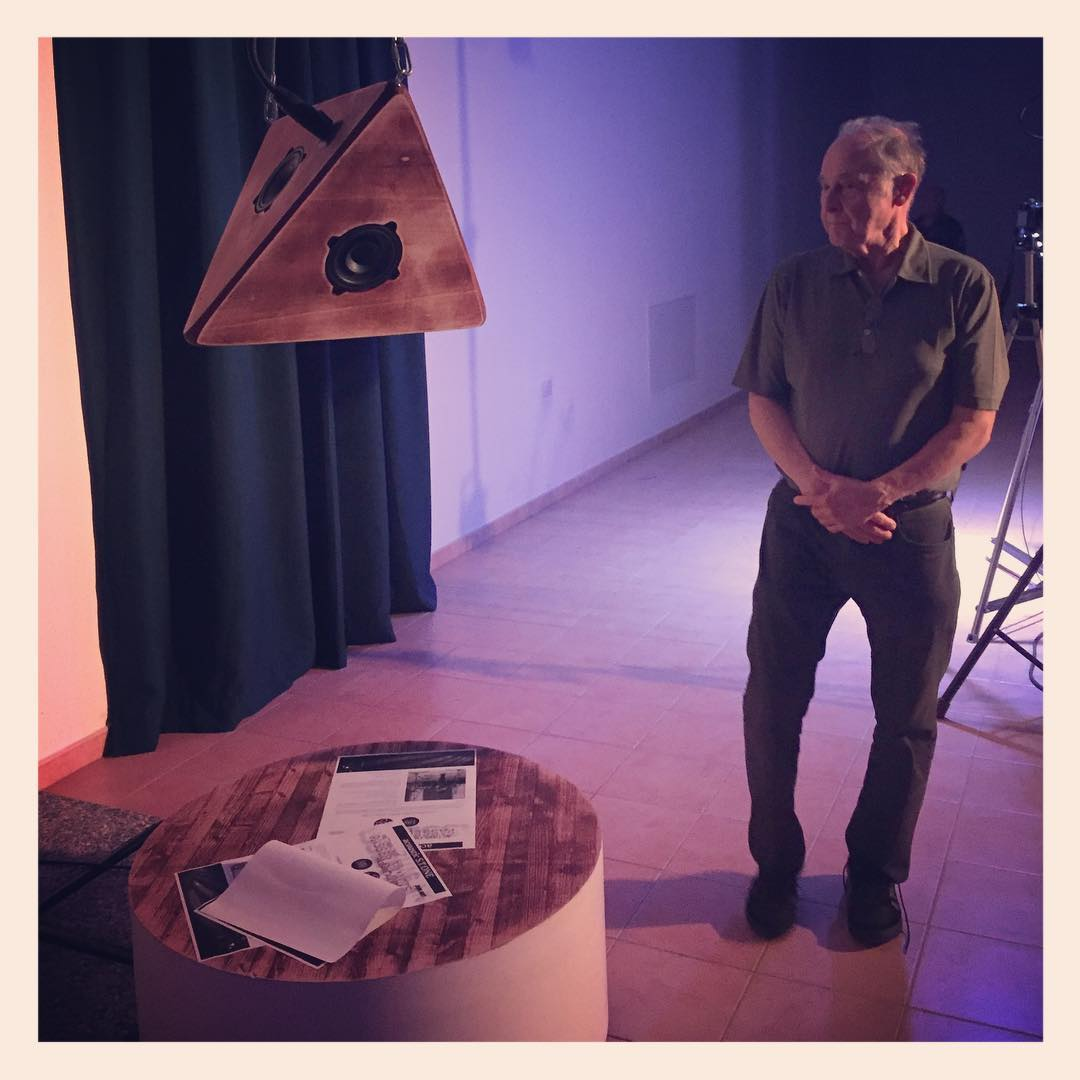
\includegraphics[width=.47\textwidth]{img/14597413_1128159647252783_1502048594255937536_n.jpg}
\caption{John Chowning listening \emph{ACOUSTIC STONE}, \emph{Aumentazioni Festival}, Salerno, Italy, 2016.}
\label{stone2}
\end{center}
\end{figure}

%\section*{UNISOLO}

As last stage, \emph{Unisolo} is a composition for four ensembles. Through writing it I will investigate the role of shape in a shape-informed dialogue with the listener. 
%at the depth of every literature, the time

%\onecolumn
\bibliographystyle{plain}
\bibliography{ttt.bib}

~

\vfill

\begin{figure}[htbp]
\centering
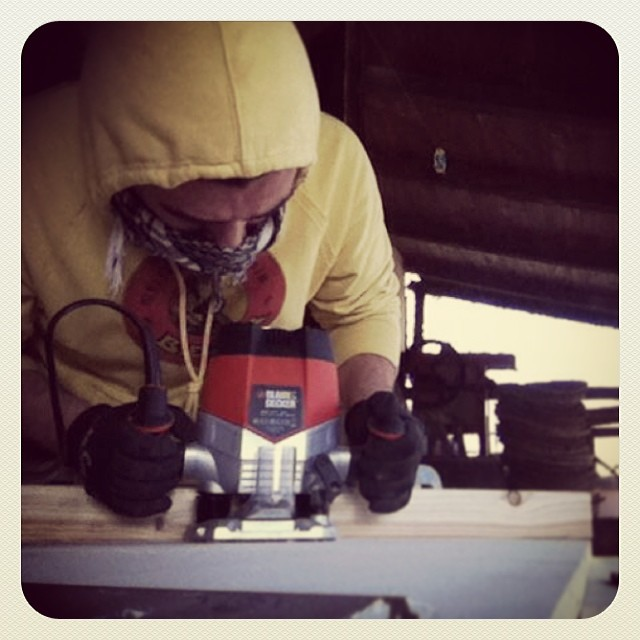
\includegraphics[width=.47\textwidth]{img/927576_1422938657945799_34474354_n}
\caption{Giuseppe Silvi. Composer.}
\label{conc}
\end{figure}

\end{document}
